\documentclass[a2paper, 12pt]{article}
\usepackage[font={huge, bf}]{caption}
\usepackage{fontspec}
\setmainfont{Arial}
\usepackage{subcaption}
\usepackage{graphicx}
\usepackage{tikz}
\usepackage{tikzsymbols}
\usetikzlibrary{calc,patterns,shapes.geometric}
\usepackage{float}
\usepackage{pdflscape}
\usepackage{geometry}
\geometry{landscape, margin=2cm}
\captionsetup[subfigure]{justification=justified,singlelinecheck=false}
\pagestyle{empty}

\def\centerarc[#1](#2)(#3:#4:#5){\draw[#1] ($(#2)+({#5*cos(#3)},{#5*sin(#3)})$) arc (#3:#4:#5);}

\begin{document}
	\vspace*{\fill}
	\begin{figure}[!htbp]
		\centering
		\begin{subfigure}[b]{0.48\textwidth}
			\caption{Figure 1}
			\centering
			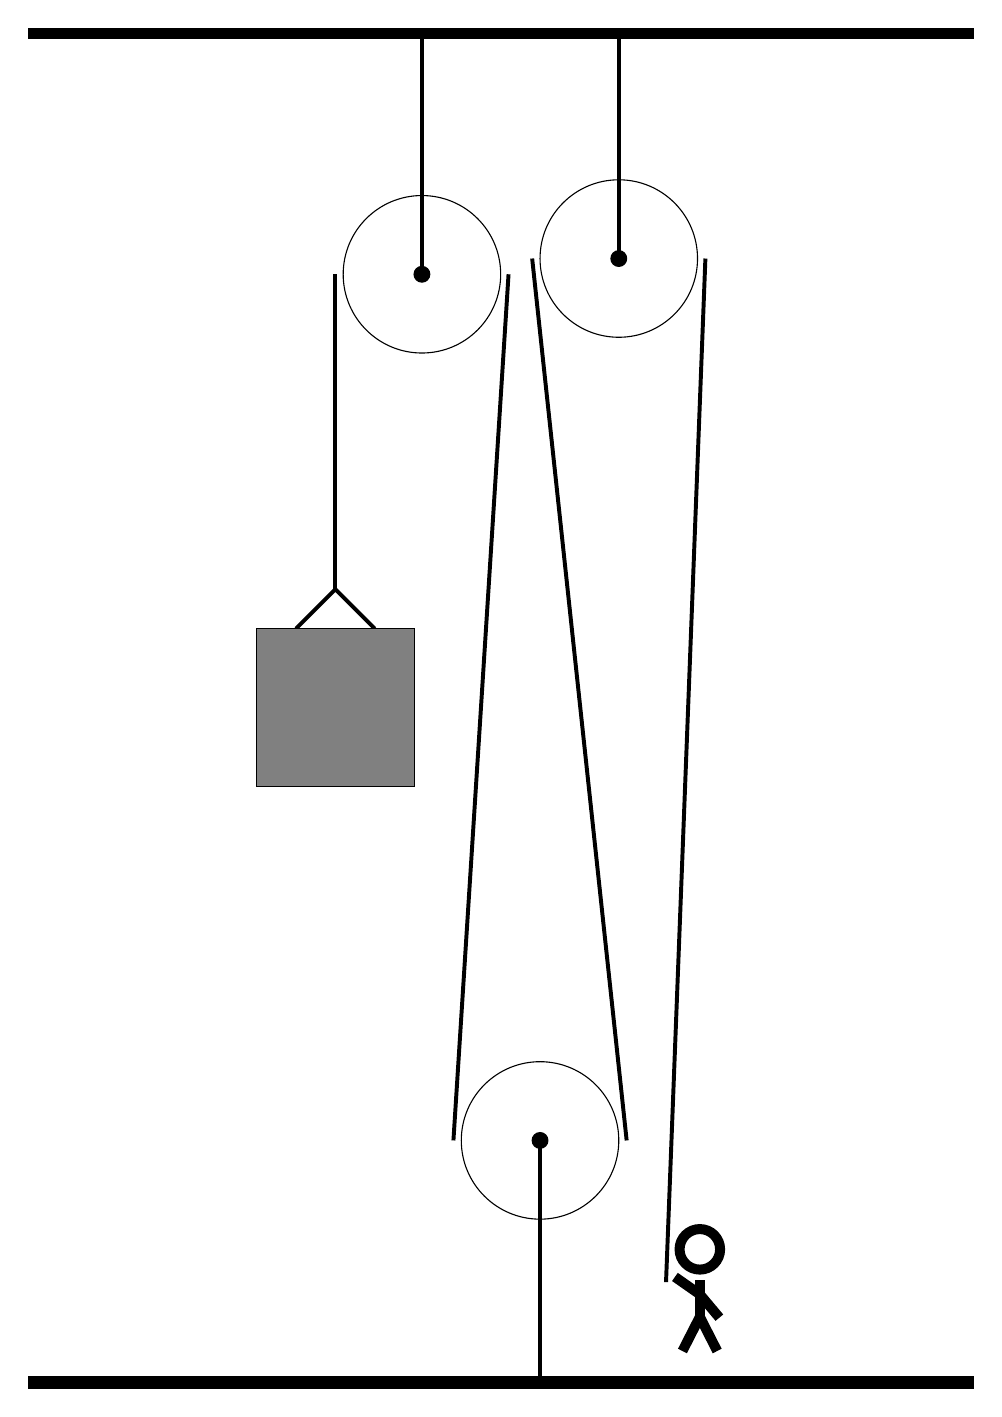
\begin{tikzpicture}
				\draw[fill=black] (-4, 14) rectangle (8, 14.125);
				
				\draw (1, 11) circle (1);
				\draw[fill=black] (1, 11) circle (0.1);
				\draw[line width=0.5mm]  (1, 14) -- (1, 11);
				
				\draw[fill=white](2.5, 0) circle (1);
				\draw[fill=black] (2.5, 0) circle (0.1);
				\draw[line width=0.5mm]  (2.5, -3) -- (2.5, 0);
				
				\draw[fill=white](3.5, 11.2) circle (1);
				\draw[fill=black] (3.5, 11.2) circle (0.1);
				\draw[line width=0.5mm] (3.5, 14) -- (3.5, 11.2);
				
				\draw[line width=0.5mm] (-0.6, 6.5) -- (-0.1, 7.0) -- (0.4, 6.5);
				\draw[fill=black!50] (-1.1, 6.5) rectangle (0.9, 4.5);
				
				\draw[line width=0.5mm] (-0.1, 11) -- (-0.1, 7.0);
				\centerarc[line width=0.5mm](1, 11)(0:180:1.1);
				\draw[line width=0.5mm](2.1, 11) -- (1.4, 0);
				\centerarc[line width=0.5mm](2.5, 0)(180:360:1.1);
				\draw[line width=0.5mm](3.6, 0) -- (2.4, 11.2);
				\centerarc[line width=0.5mm](3.5, 11.2)(0:180:1.1);
				\draw[line width=0.5mm](4.6, 11.2) -- (4.1, -1.8);
				
				\node at (4.5, -1.9) {\scriptsize \Strichmaxerl[10][-35][-50]};
				
				\draw[fill=black] (-4, -3) rectangle (8, -3.15);
			\end{tikzpicture}
		\end{subfigure}
		\hfill
		\begin{subfigure}[b]{0.48\textwidth}
			\caption{Figure 2}
			\centering
			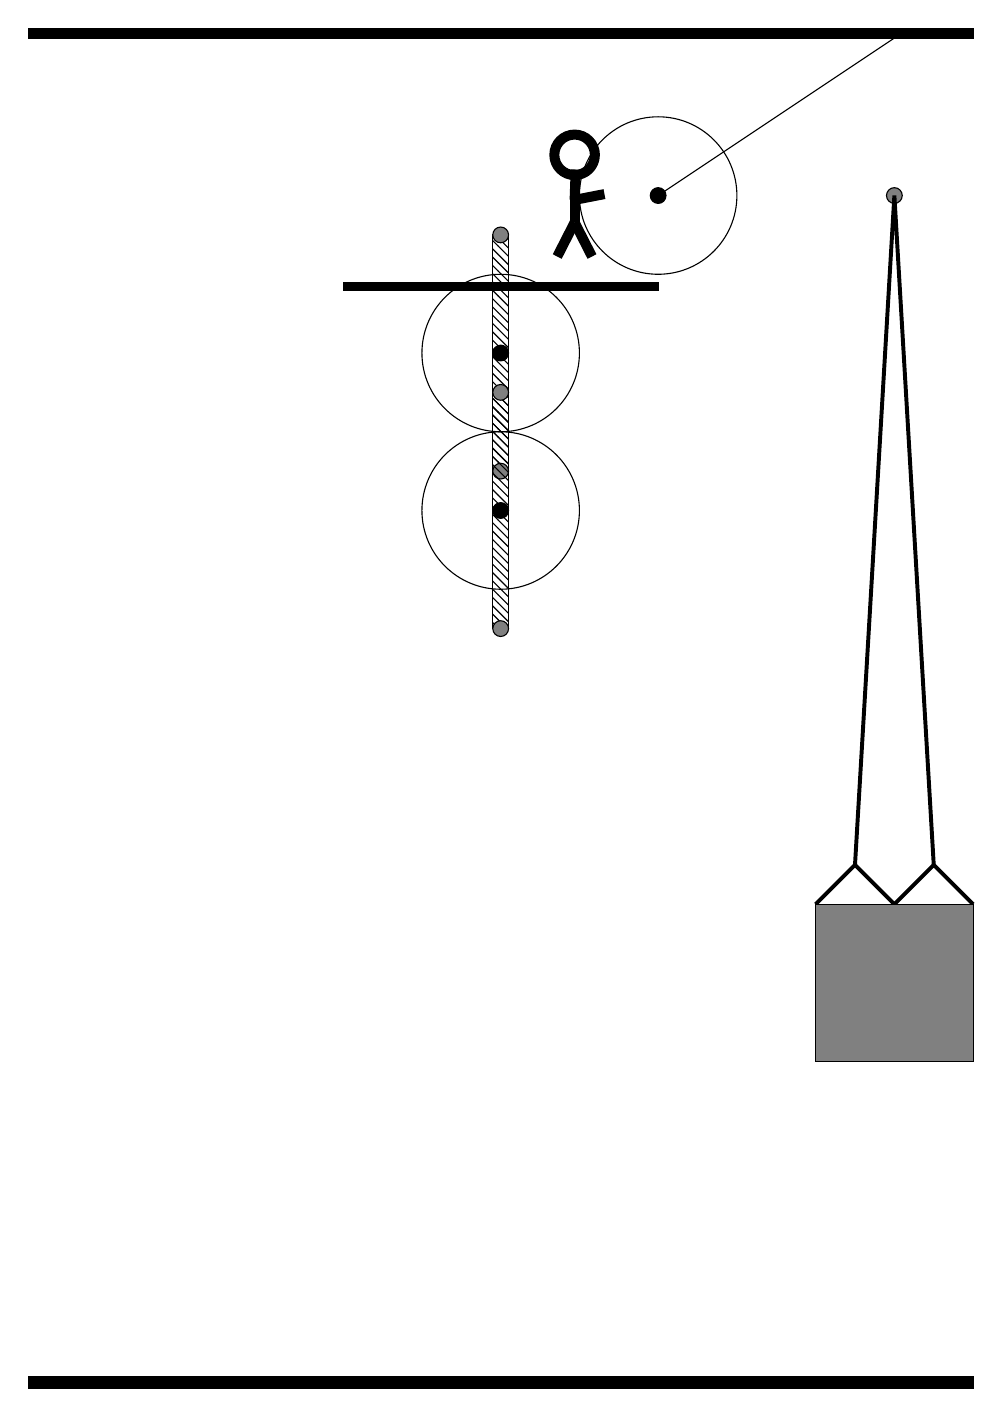
\begin{tikzpicture}
				\draw[fill=black] (-4, 14) rectangle (8, 14.125);
				
				\draw (2,10) circle (1);
				\draw[fill=black] (2,10) circle (0.1);
				\draw[pattern=north west lines, pattern color=black] (1.9,11.5) rectangle (2.1,8.5);
				\draw[fill=black!50] (2,11.5) circle (0.1);
				\draw[fill=black!50] (2,8.5) circle (0.1);
				
				\draw (2,8) circle (1);
				\draw[fill=black] (2,8) circle (0.1);
				\draw[pattern=north west lines, pattern color=black] (1.9,9.5) rectangle (2.1,6.5);
				\draw[fill=black!50] (2,9.5) circle (0.1);
				\draw[fill=black!50] (2,6.5) circle (0.1);
				
				\draw (4,12) circle (1);
				\draw[fill=black] (4,12) circle (0.1);
				\draw (7,14.0) -- (4,12);
				
				\draw[fill=black!50] (7,12) circle (0.1);
				\draw[line width=0.5mm](6.5,3.5) -- (7,12) --  (7.5,3.5);
				\draw[line width=0.5mm](6,3) --  (6.5,3.5) -- (7,3) -- (7.5,3.5) -- (8,3);
				\draw[fill=black!50] (6, 3) rectangle (8, 1);
				
				
				\node at (3, 12) {\scriptsize \Strichmaxerl[10][-92][11]};
				\draw[fill=black] (0, 10.9) rectangle (4, 10.8);
				
				\draw[fill=black] (-4, -3) rectangle (8, -3.15);
			\end{tikzpicture}
		\end{subfigure}
	\end{figure}
		\vspace*{\fill}
\end{document}